\chapter{Diseño e Implementación}

\section{Arquitectura Cliente-Servidor}

El proyecto en general está basado en la arquitectura cliente-servidor\cite{clienteservidor}. Esta arquitectura, como su nombre indica, define dos roles principales que se reparten tareas de demanda y respuesta: cliente y servidor. Esta separación se produce en nuestro proyecto cuando distinguimos entre \textit{front-end} (cliente) y nuestro \textit{back-end} (servidor).

la interfaz haría las funciones de cliente, siendo la demandante de información; por otro lado la API junto con la base de datos tendrían el rol de servidor, encargado de procesar las peticiones y responder de manera adecuada a la petición original.

Con esta disposición se puede destacar la ventaja de que al tener bien diferenciado el \textit{back-end}, la aplicación será adaptable a cualquier tipo de \textit{front-end}. Además, la función de mantenimiento es mucho más fácil de llevar a cabo en este tipo de arquitecturas, pues si aparece algún problema en la parte de interfaz, se puede corregir sin que la modificación aplicada altere el funcionamiento de nuestro \textit{back-end} o API.

\subsection{Arquitectura Cliente-Servidor y Modelo-Vista-Controlador}

Aún cuando estas dos arquitecturas no son incompatibles, tal y como se ha comentado en la sección \ref{sec::arquitecturaMVC}, en este proyecto se han diferenciado tres bloques distintos, basados en el \textit{MVC}, con funciones asignadas: vista, controlador y modelo. 

Una vez desarrollados esos bloques, la arquitectura cliente-servidor se engloba en un solo bloque, llamando servidor a los bloques: controlador y modelo. La función que esta arquitectura entiende por servidor es la que se realizaría gracias a la unión de estos dos bloques.

\section{Diseño}

El diseño es un proceso que permite construir una representación abstracta del software de forma que se puedan conocer aspectos como la arquitectura, funcionalidades o la calidad antes de comenzar la codificación. Además, permite detectar problemas en etapas muy tempranas del proyecto, ahorrando costes y reduciendo la presencia de riesgos. En SCRUM el diseño del software es continuo y se actualiza en cada \textit{sprint}.

A continuación se mencionan algunos aspectos del diseño de la aplicación que resultan interesantes o relevantes para el correcto funcionamiento.

\subsection{Representación de los datos}

Los datos serán representados en nuestro bloque o módulo que actuará como vista. Para ello, como ya describimos en sección \ref{sec::analisis_vistaInterfaz}, lo desarrollaremos usando el \textit{framework} ReactJS.

Los datos tienen que mostrarse en una interfaz que sea sencilla de usar, intuitiva y que se adapte a todo tipo de navegadores. Para la elección del aspecto de la misma, es necesaria la búsqueda de inspiración. Por lo que la interfaz de la aplicación Instagram\footnote{https://www.instagram.com/?hl=es} ha sido considerada como modelo a seguir. Observando esta interfaz en la figura \ref{fig::insta}, se puede comprobar que, en cualquier momento, un usuario tiene la posibilidad de cambiar la vista general gracias a los 4 botones que contiene en el extremo inferior de la pantalla. Esta funcionalidad, será clave a la hora de buscar una plantilla que ayude para el inicio del desarrollo de la interfaz pues en nuestro diseño será fundamental que el usuario tenga la posibilidad de desplazarse por los distintos apartados de la aplicación siempre que lo necesite.

\begin{figure}[htbp]
    \centerline{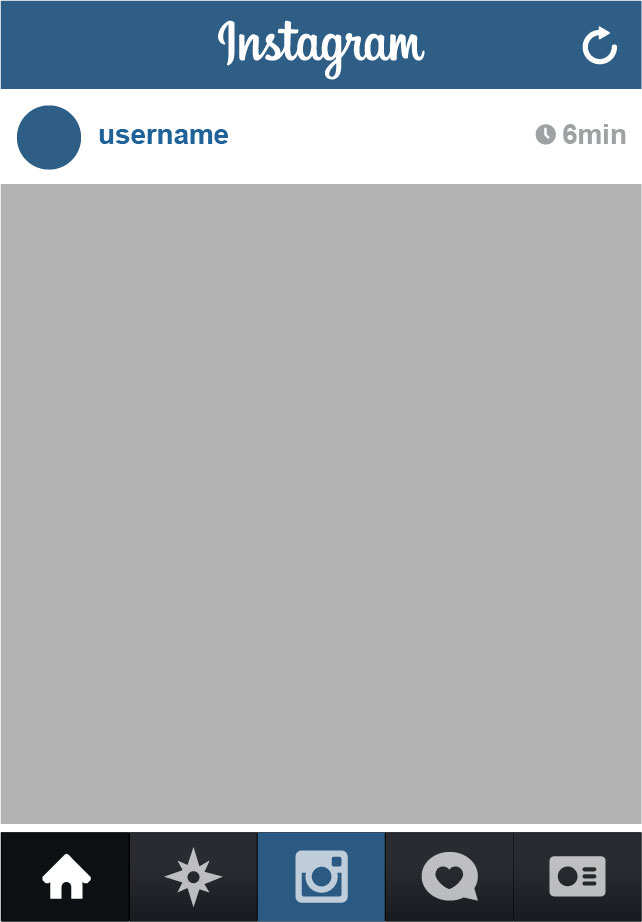
\includegraphics[width=4cm]{figuras/insta.jpg}}
    \caption{Interfaz de Instagram}
    \label{fig::insta}
\end{figure}

La idea principal es la reutilización de código con licencia de código abierto. Gracias a la comunidad de software libre, se ha encontrado una interfaz que relacione la idea descrita anteriormente junto con un diseño sencillo e intuitivo. Esta plantilla se llama \textbf{adminLTE}\footnote{https://github.com/almasaeed2010/AdminLTE}, está liberada bajo la licencia de software libre \textit{MIT}\footnote{https://github.com/almasaeed2010/AdminLTE/blob/master/LICENSE} y se encuentra alojada en la plataforma GitHub.

Gracias al uso de la misma, se ha podido desarrollar una interfaz sencilla de desarrollar y agradable a la vista. En la imagen \ref{fig::rid} se puede observar como se ha desarrollado una interfaz en la que un usuario puede, en cualquier momento, cambiar el contenido de la vista principal.

\begin{figure}[htbp]
    \centerline{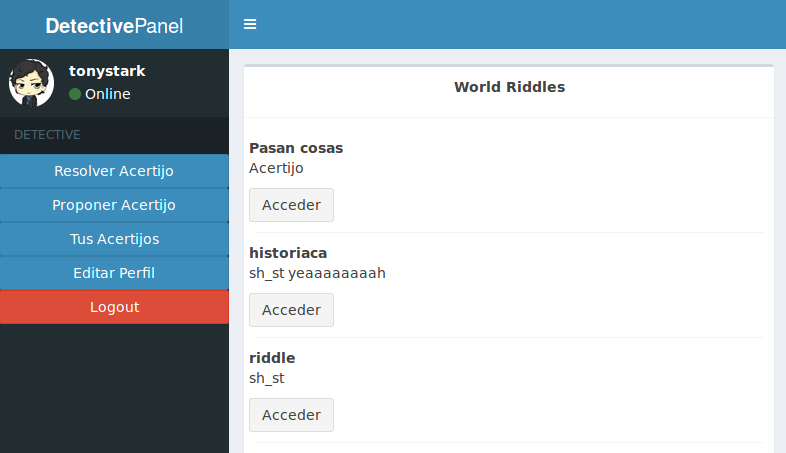
\includegraphics[width=12cm]{figuras/riddling.png}}
    \caption{Interfaz de Riddling, nuestro proyecto}
    \label{fig::rid}
\end{figure}

\subsubsection{ReactJS y sus componentes}

ReactJS es un \textit{framework} que se basa en la reutilización de componentes. Un componente es cualquier estructura definida en la que se mostrará información. Cada componente se comporta como una instancia de una clase, por lo que cada uno de ellos tiene sus atributos definidos.

El procedimiento a seguir para la creación de la vista consiste en el diseño y desarrollo de las 4 vistas iniciales que dispondrá la aplicación:

\begin{itemize}
    \item \textbf{AcertijosView}. En esta sección se mostrarán todas las historias accesibles del sistema. Esta vista contendrá todos los componentes \textit{SmallRiddle} que posteriormente describiremos. Esta vista se puede observar en la figura \ref{fig::acertijosview}.
    \item \textbf{ProponerView}. En este apartado se mostrará un formulario para que un usuario introduzca un acertijo. Esta vista se puede observar en la figura \ref{fig::proponerview}.
    \item \textbf{TusAcertijosView}. En este apartado se mostrarán todas las historias propias de un usuario. Esta vista también contendrá todos los componentes \textit{SmallRiddle} que posteriormente describiremos. Esta vista se puede observar en la figura \ref{fig::tusacertijosview}.
    \item \textbf{EditarPerfilView}. Gracias a esta vista un usuario será capaz de administrar su perfil. Aparecerá un formulario con los datos que podrá modificar. Nótese que esta interfaz se encuentra diseñada pero actualmente se encuentra sin funcionalidad. Se puede observar en la figura \ref{fig::editarperfilview}.
\end{itemize}

\begin{figure}[hbtp] \centering
\begin{subfigure}{.8\textwidth}
    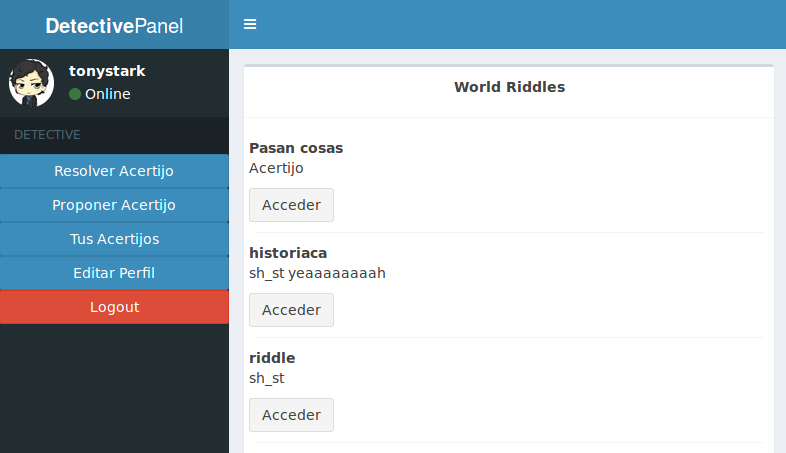
\includegraphics[width=\linewidth]{figuras/riddling.png}
    \caption{Vista AcertijosView de la aplicación}
    \label{fig::acertijosview}
\end{subfigure}
\begin{subfigure}{.8\textwidth}
    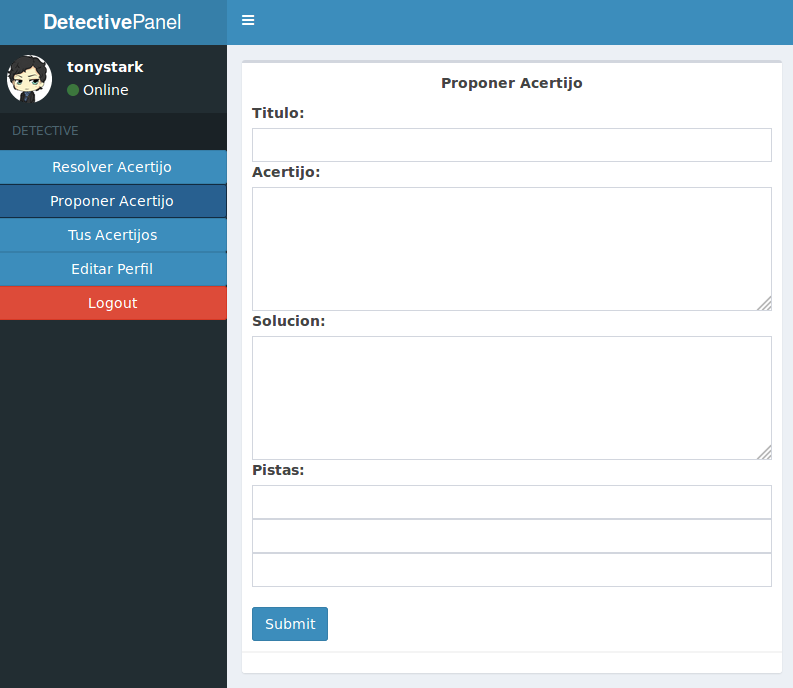
\includegraphics[width=\linewidth]{figuras/proponerview.png}
    \caption{Vista ProponerView de la aplicación}
    \label{fig::proponerview}
\end{subfigure}
\caption{Imágenes de las vistas que componen la aplicación}
\end{figure}

\begin{figure}[htbp]\ContinuedFloat
\centering
\begin{subfigure}{.8\textwidth}
    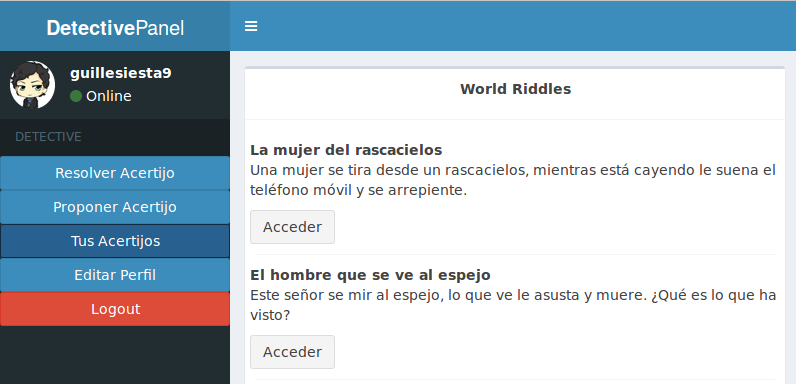
\includegraphics[width=\linewidth]{figuras/tusacertijosview.png}
    \caption{Vista de TusAcertijosView de la aplicación}
    \label{fig::tusacertijosview}
\end{subfigure}
\begin{subfigure}{.8\textwidth}
    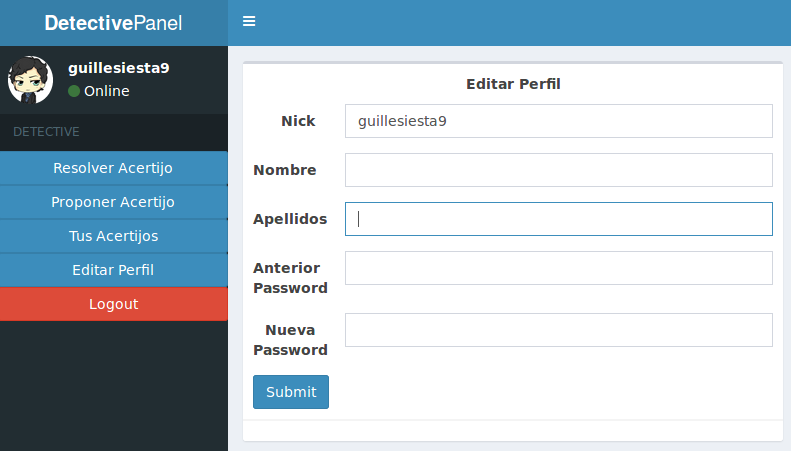
\includegraphics[width=\linewidth]{figuras/editarperfilview.png}
    \caption{Vista de EditarPerfilView de la aplicación} 
    \label{fig::editarperfilview}
\end{subfigure}
\caption{Imágenes de las vistas que componen la aplicación}
\label{fig::vistas}
\end{figure}
Una vez definidas las vistas, éstas contendrán distintos tipos de componentes que interactuarán entre ellos para poder realizar las funciones descritas en los requisitos de la aplicación. Estos componentes se dividen en:

\begin{itemize}
    \item \textbf{Header}. En este componente encontramos la cabecera de la aplicación. Contiene un botón que al pulsarlo contrae hacia la izquierda el menú \textit{Sidebar}. Está siempre renderizado.
    \item \textbf{Sidebar}. Este componente es el encargado de seleccionar qué vista es la que queremos escoger y visualizar. Este componente se encuentra siempre accesible.
    \item \textbf{FormLogin}. El componente inicial que nos permite acceder a la plataforma mediante un usuario y una contraseña.
    \item \textbf{SmallRiddle}. Es un componente que resume el título del acertijo y la descripción del mismo. Tenemos la posibilidad de acceder a él para así cargar el componente \textit{Riddle}.
    \item \textbf{Riddle}. Muestra todos los datos del acertijo, a excepción de la solución. Este componente nos permite observar el estado en el que se encuentra el acertijo, la descripción del mismo, y las tres valiosas pistas que nos ayudarán a resolverlo.
    
    Como funcionalidad adicional, este componente puede cargar todas las soluciones propuestas de ese acertijo  por los usuarios y el porcentaje de cercanía con respecto a la solución final.
    \item \textbf{Solución}. Componente que muestra el texto de la propuesta como solución de un acertijo y la puntuación otorgada por el creador del acertijo.
    \item \textbf{SolucionConCheck}. Este componente muestra la solución de un acertijo en concreto, y tiene la posibilidad de poder establecer una puntuación con respecto al porcentaje de cercanía a la solución del acertijo. Este componente se renderiza únicamente en la vista \textit{TusAcertijosView}.
\end{itemize}

En la figura \ref{fig::componentes} se puede observar el aspecto de cada uno de los componentes descritos.

\begin{figure}[hbtp] \centering
\begin{subfigure}{.6\textwidth}
     \centerline{
\includegraphics[width=8cm]{figuras/header.png}}
    \caption{Componente Header de la aplicación}
    \label{fig::header}
\end{subfigure}
\par\bigskip 
\begin{subfigure}{.6\textwidth}
    \centerline{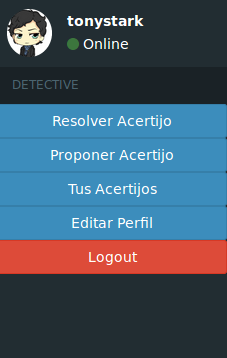
\includegraphics[width=5cm]{figuras/sidebar.png}}
    \caption{Componente Sidebar de la aplicación}
    \label{fig::sidebar}
\end{subfigure}
\par\bigskip 
\begin{subfigure}{.6\textwidth}
     \centerline{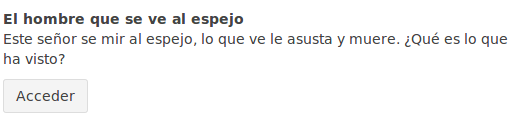
\includegraphics[width=9cm]{figuras/smallriddle.png}}
    \caption{Componente SmallRiddle de la aplicación}
    \label{fig::smallriddle}
\end{subfigure}
\caption{Imágenes de los componentes que componen la aplicación}
\end{figure}
\begin{figure}[hbtp] \centering \ContinuedFloat
\begin{subfigure}{.6\textwidth}
     \centerline{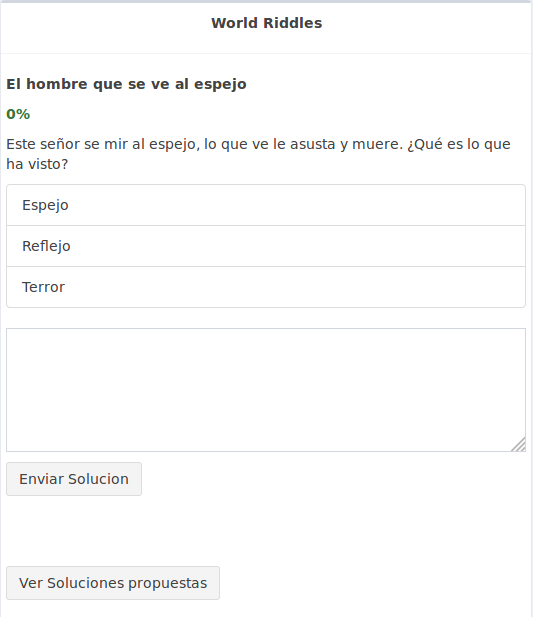
\includegraphics[width=9cm]{figuras/riddle.png}}
    \caption{Componente Riddle de la aplicación} 
    \label{fig::riddle}
\end{subfigure}
\par\bigskip 
\begin{subfigure}{.6\textwidth}
     \centerline{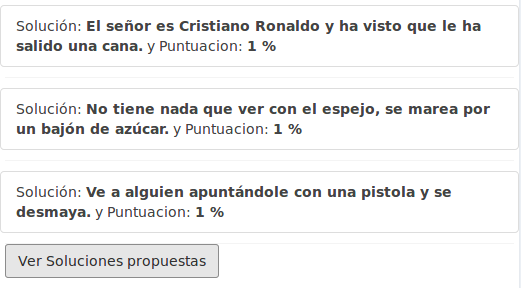
\includegraphics[width=9cm]{figuras/solucion.png}}
    \caption{Componente Solución de la aplicación} 
    \label{fig::solucionComponent}
\end{subfigure}
\par\bigskip 
\begin{subfigure}{.6\textwidth}
     \centerline{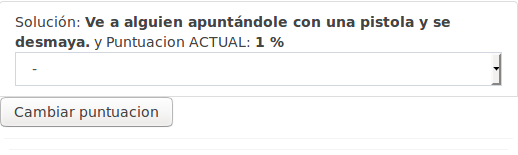
\includegraphics[width=9cm]{figuras/solucionconcheck.png}}
    \caption{Componente SoluciónConCheck de la aplicación} 
    \label{fig::solucionconcheck}
\end{subfigure}
\caption{Imágenes de los componentes que componen la aplicación}
\label{fig::componentes}
\end{figure}


\subsection{Modulado de los datos}

En esta aplicación se van a distinguir dos tipos de entidades: usuarios y acertijos. Esto, en términos de la base de datos basada en grafos, corresponde a dos tipos de nodos específicos: \textbf{Usuarios} y \textbf{Storie}.


Se representan en la base de datos tal y como se muestra en la figura \ref{fig::nodos}. 

\begin{figure}[hbtp] \centering
\begin{subfigure}{.6\textwidth}
     \centerline{
\includegraphics[width=2cm]{figuras/usuario.png}}
    \caption{Nodo Usuario} 
    \label{fig::usernode}
\end{subfigure}
\begin{subfigure}{.6\textwidth}
     \centerline{
\includegraphics[width=2cm]{figuras/storie.png}}
    \caption{Nodo Storie} 
    \label{fig::storynode}
\end{subfigure}
\caption{Nodos de la base de datos }
\label{fig::nodos}
\end{figure}

\subsubsection{Atributos del usuario}

En la base de datos se almacenarán los siguientes atributos por nodo usuario:

\begin{itemize}
    \item \textbf{Nick}.
    \item \textbf{Contraseña}.
    \item \textbf{Nombre}.
    \item \textbf{Apellidos}.
\end{itemize}


\subsubsection{Atributos del acertijo}
En la base de datos se almacenarán los siguientes atributos por nodo Storie:

\begin{itemize}
    \item \textbf{Título}.
    \item \textbf{Sh\_Storie}. (acertijo)
    \item \textbf{Storie}. (solución)
    \item \textbf{Pista 1}.
    \item \textbf{Pista 2}.
    \item \textbf{Pista 3}.
\end{itemize}

\subsubsection{Relaciones entre nodos}

En el sistema se distinguen dos tipos de relaciones:

\begin{itemize}
    \item \textbf{Escribe}. Relacionará cuando un usuario escribe un acertijo.
    \item \textbf{Propone}. Relacionará cuando un usuario propone una solución a un acertijo.
\end{itemize}

Una vez se establece el tipo de relaciones existentes en el sistema y se decida crear una relación \textit{Usuario escribe historia}, la representación gráfica sería la que se muestra en la figura \ref{fig::escribe}.

\begin{figure}[hbtp]
     \centerline{
\includegraphics[width=5cm]{figuras/escribe.png}}
    \caption{Relación (Usuario)-[Escribe]-(Storie)} 
    \label{fig::escribe}
\end{figure}

Neo4j nos ofrece la posibilidad de poder añadir atributos a las relaciones. Esto será útil para la relación \textit{Propone}, pues en esa relación será necesario registrar el texto propuesto como solución y la puntuación de esa propuesta (inicialmente será de 1). Esta relación quedaría representada tal y como describe la figura \ref{fig::propone}.

\begin{figure}[hbtp]
     \centerline{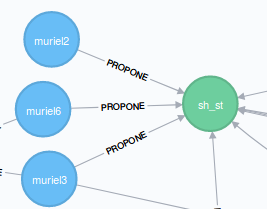
\includegraphics[width=5cm]{figuras/propone.png}}
    \caption{Relación (Usuario)-[Propone]-(Storie)} 
    \label{fig::propone}
\end{figure}

\subsubsection{Conclusión sobre el modelado de grafos y su consulta}

Como se puede observar, es realmente intuitiva y sencilla la representación gráfica que este tipo de base de datos nos propone. Sin embargo, más sencillo  en intuitivo es aún el lenguaje Cypher necesario para la realización de consultas. Pues éste, con una breve ojeada a su manual de usuario\footnote{https://neo4j.com/docs/developer-manual/current/cypher/}, ya se es capaz de realizar cualquier tipo de consulta necesaria para el funcionamiento de la aplicación. Por ejemplo, en el caso de que necesitásemos extraer de la base de datos todos los acertijos propuestos por el usuario ``aristoteles'', la consulta sería la siguiente:
\begin{flushleft}
    \texttt{MATCH (u:Usuario)-[r:Escribe]-(s:Storie)\\ WHERE u.nick=aristoteles\\ RETURN s.storie}

\end{flushleft}

\subsection{Control de los datos}

Esta aplicación tiene que garantizar que todos los datos enviados y recibidos por los componentes o la base de datos son gestionados de manera adecuada. Es por ello que el controlador implementa una serie de métodos  que aseguran la integridad de los datos y que se invocan desde la interfaz.

Este controlador debe de estar conectado a la base de datos, y tiene que ser apto al recibo de peticiones por parte de la interfaz. Además, deberá limitarse única y exclusivamente a la ejecución de esos métodos, por lo que necesitamos que sea un servicio ligero. Flask nos garantiza todo lo anterior.

Nuestro controlador tendrá los siguientes métodos:

\begin{itemize}
    \item \textbf{all\_stories\_titulo()}. Devuelve todos los títulos de las historias del sistema.
    \item \textbf{user\_stories\_titulo()}. Devuelve los títulos de las historias creadas por un usuario en concreto.
    \item \textbf{soluciones\_por\_titulo()}. Devuelve todas las soluciones propuestas para un acertijo y su puntuación.
    \item \textbf{enviar\_comentario()}. Se añade en la base de datos la propuesta de solución de un usuario para un acertijo en concreto.
    \item \textbf{enviar\_storie()}. Se añade en la base de datos un acertijo.
    \item \textbf{cambiar\_puntuacion\_titulo()}. Se modifica en la base de datos la puntuación de una posible solución de un acertijo. Una vez cambiada la puntuación, se procederá a la actualización del estado del acertijo buscando cuál es la mayor puntuación que existe de las soluciones propuestas.
    \item \textbf{acertijo\_por\_titulo()}.Devuelve el acertijo que coincide con un título especifico, así como el texto del mismo.
    \item \textbf{storie\_por\_titulo()}.Devuelve el acertijo que coincide con un título especifico y  la solución del mismo.
    \item \textbf{todo\_por\_titulo()}.Devuelve el acertijo que coincide con un título especifico y todos sus atributos.
    \item \textbf{login()}. Se busca en la base de datos si el usuario existe y la contraseña coincide con la registrada en el sistema.
\end{itemize}

\subsection{Flujo de los datos}

El flujo de datos puede ir desde la interfaz hasta la base de datos y viceversa. Para que esto ocurra, se usa el controlador como intermediario. 

El formato de los datos estará estructurado en JSON\footnote{https://www.json.org/}, debido a su alto uso en peticiones y respuestas mediante el protocolo HTTP.  Esto es, en el caso de que desde la interfaz decidamos añadir un acertijo, desde ahí se enviarán en formato JSON todos los datos al controlador, que posteriormente extraerá la información relevante de ese JSON y la añadirá a la base de datos.

Un ejemplo de flujo de datos y pasos a seguir es el descrito en los diagramas de secuencia de la figura \ref{fig::secuencia}. En estos diagramas se describe el funcionamiento de los eventos \textit{enviar\_storie(), enviar\_comentario(),} en las que un usuario introduce un nuevo acertijo en el sistema.

\begin{figure}[hbtp] \centering
\begin{subfigure}{.6\textwidth}
     \centerline{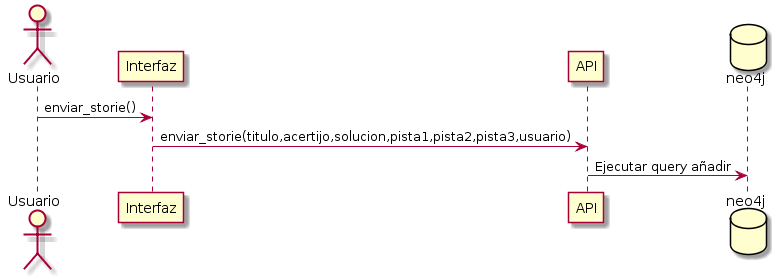
\includegraphics[width=11cm]{figuras/enviar_storie.png}}
    \caption{Diagrama de secuencia del evento enviar\_storie()} 
    \label{fig::enviarstorie}
\end{subfigure}
\begin{subfigure}{.6\textwidth}
     \centerline{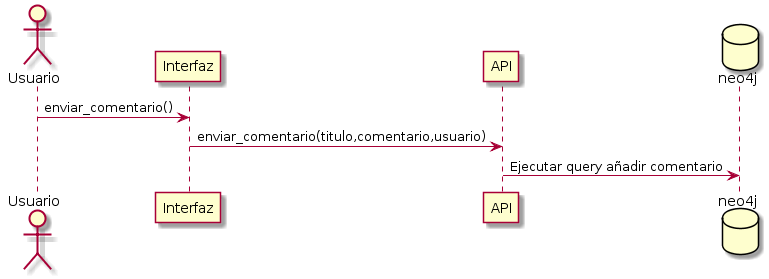
\includegraphics[width=11cm]{figuras/enviar_comentario.png}}
    \caption{Diagrama de secuencia del evento enviar\_comentario()} 
    \label{fig::enviarcomentario}
\end{subfigure}
\begin{subfigure}{.6\textwidth}
     \centerline{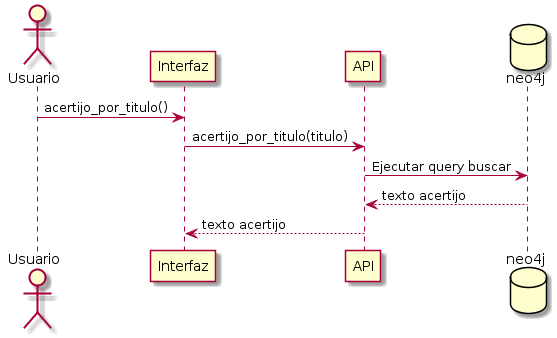
\includegraphics[width=11cm]{figuras/acertijo_por_titulo.png}}
    \caption{Diagrama de secuencia del evento acertijo\_por\_titulo()} 
    \label{fig::acertijoportitulo}
\end{subfigure}
\begin{subfigure}{.6\textwidth}
     \centerline{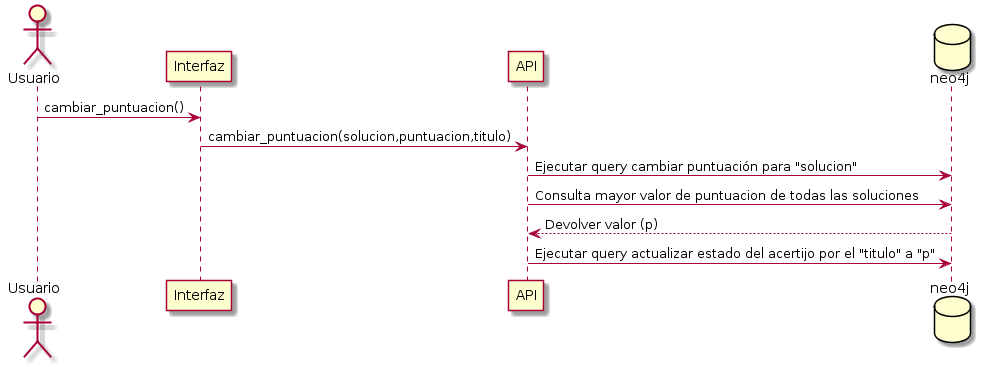
\includegraphics[width=11cm]{figuras/cambiar_puntuacion.png}}
    \caption{Diagrama de secuencia del evento cambiar\_puntuacion()} 
    \label{fig::cambiarpuntuacion}
\end{subfigure}
\caption{Diagramas de flujo de algunos eventos de la aplicación }
\label{fig::secuencia}
\end{figure}


\section{Implementación}

Una vez descrito el funcionamiento de la aplicación, el siguiente paso es la implementación. Se distinguen dos fases a la hora de llevar a cabo esta etapa. En primer lugar, se desarrollará la aplicación en la máquina local y  posteriormente, se desarrollarán los automatismos necesarios para el despliegue de la aplicación.

\subsection{Implementación en local}

Para la implementación de la aplicación en local se han implementado los tres bloques de una manera independiente, comenzando por la instalación de la base de datos, siguiendo por la creación de la API y la conexión con la anterior, hasta la creación de la interfaz.

\subsubsection{Base de datos}

Para ello, en primer lugar se ha instalado la base de datos neo4j siguiendo el tutorial oficial. Tras realizar todos los pasos, se podría acceder a la base de datos en la dirección\textit{localhost://7474}, asignada por defecto\cite{neo4jinstall}.

\subsubsection{API}

Para la creación de la API REST, se ha usado Flask, y se ha implementado este servicio de una manera cómoda y sencilla. Simplemente se ha ejecutado el comando \texttt{python nuestraapi.py}, que arranca el servicio local, accesible por el puerto 5000\cite{flaskinstall}.

\subsubsection{Interfaz}

Para el desarrollo de la interfaz se ha seguido el tutorial oficial para el inicio y la instalación de ReactJS\cite{reactinstall}. Este proceso se debe arrancar y por defecto se situará en local en el puerto 3000.

\subsubsection{Conectando interfaz, controlador y modelo}

Una vez desarrollado cada bloque, es necesario establecer una conexión para crear el cauce por donde fluirá la información.

Para ello, en la API se debe establecer primero la conexión mediante las claves ofrecidas por la base de datos\cite{connectflaskneo4j}. Posteriormente, se debe instalar la librería Py2neo\footnote{https://py2neo.org/v4/} que, recomendada por la documentación oficial de neo4j, sera de ayuda a la hora de hacer consultas y establecer la conexión con la base de datos.

Una vez esté el \textit{back-end} conectado entre sí (API+Neo4j), será necesario conectarlo con la interfaz.

En este sentido, una de las ventajas de javascript (el lenguaje oficial para la interfaz) es que dispone de una función \textit{fetch}\footnote{https://developer.mozilla.org/es/docs/Web/API/Fetch\_API/Utilizando\_Fetch}, que se encargará de realizar las peticiones HTTP a la API. 

\subsection{Implementación en la nube}

A la hora de implementar en la nube, se seguirá el mismo orden que en local. 

\subsubsection{Base de datos}
En primer lugar, es necesario darse  de alta en la plataforma GrapheneDB\footnote{https://www.graphenedb.com/}. Previamente exportada la base de datos en local (en el caso de que se quiera mantener la información) se procede a la creación de una nueva base de datos en GrapheneDB. Una vez creada, se restaura la nueva creación con los datos exportados de la base de datos en local\cite{graphenedb}.

Siguiendo estos sencillos pasos, ya estaría la base de datos desplegada en la nube.


\subsubsection{API REST}

Para el despliegue de la API REST en la plataforma Zeit\footnote{https://zeit.co/} primero es necesario especificar qué entorno se construirá. Para ello, es necesario crear dos archivos:

\begin{itemize}
    \item \textbf{requirements.txt}\footnote{https://github.com/guillesiesta/ProjectX/blob/master/requirements.txt}. Este archivo define un entorno mediante el cual la aplicación podrá ejecutar Python.
    
    \item \textbf{Dockerfile}\footnote{https://github.com/guillesiesta/ProjectX/blob/master/Dockerfile}. Este archivo,  define un entorno en el cual Zeit podrá crear un contenedor donde alojar el servicio.
\end{itemize}

Una vez creados estos archivos, se debe comunicar en la API que dejará de comunicarse por el puerto 5000 y pasará a comunicarse por el puerto 80. Para ello, habrá que añadir la siguiente línea al final del documento: \textit{app.run(host='0.0.0.0', port=80)}.

Una vez efectuados los cambios, se ejecuta desde el directorio de la aplicación el comando: \texttt{now --public} y comenzará automáticamente el despliegue. 

Zeit crea nombres de dominio aleatorios, en este caso el nombre de dominio, es decir, la API o servicio estará desplegada en el dominio: \textbf{https://projectx-wvueafqhpp.now.sh/}

\subsubsection{Interfaz}

Para el despliegue en Heroku de la interfaz, es necesario instalar primero el cliente en local\cite{heroku}. Además, antes del despliegue es necesario cambiar la dirección de todas las funciones \texttt{fetch}, pues la API ahora estará alojada en la nube, y es la que se usará.

Una vez realizados los cambios correspondientes e instalado el cliente, se añadirá el repositorio local a los repositorios de Heroku\cite{heroku2}. 

Por último, se puede procede al despliegue de la interfaz con el comando: \texttt{heroku create}.

Automáticamente se desplegará una aplicación a la que, desde el panel principal de Heroku, se le podrá modificar el nombre, pero no la extensión que añade Heroku por defecto. Para tener un dominio propio se debería de escoger otro plan que no sea el gratuito.

La dirección oficial y, también la confirmación de que la aplicación está alojada en la nube es: \textbf{https://riddling.herokuapp.com/}